\documentclass{simple-article}

\usepackage{amsmath}
\usepackage{datetime2}
\usepackage{amro-common}

%%%%%%%%%%%%%%%%%%%%%%%%%%%%%%%%%%%%%%%%%%%%%%%%%%%%%%%%%%%%%%%%%%%%%%%%%%%%%%%%%%%%%%%%%%%%%%%%%%%%
%%%%%%%%%%%%%%%%%%%%%%%%%%%%%%%%%%%%%%%%%%%%%%%%%%%%%%%%%%%%%%%%%%%%%%%%%%%%%%%%%%%%%%%%%%%%%%%%%%%%

\title{Estimator's Credibility Tests}
\author{Amro Al-Baali}
\date{\today}

\bibliography{references.bib}

\renewcommand{\symProb}{P}

\graphicspath{{../}{../figs/}{figs/}}
%%%%%%%%%%%%%%%%%%%%%%%%%%%%%%%%%%%%%%%%%%%%%%%%%%%%%%%%%%%%%%%%%%%%%%%%%%%%%%%%%%%%%%%%%%%%%%%%%%%%
\begin{document}
\maketitle

\section{Introduction}
Lately, I came across this paper \cite{liEvaluationEstimationAlgorithms2012} that shows how ANEES test can fail when testing the credibility of a parameter estimate. In this document, I'll try my best to show how the ANEES test may fail; I'll show it in the context of filtering. 

\section{ANEES tests}
\subsection{Theory}
Consider a multivariate random variable $\mbfrv{x}\sim\mc{N}\left( \mbs{\mu}, \mbs{\Sigma} \right)$, where $\mbs{\mu}\in\rnums^{n_{x}}, \mbs{\Sigma}\in\rnums^{n_{x}\times n_{x}}$ are the \emph{true} parameters. 

The normalized estimation error squared (NEES) random variable is given by
\begin{align}
  \rv{\epsilon}_{i} &\coloneqq \left( \mbfrv{x}_{i} - \mbfhatrv{x}_{i} \right)^{\trans}\mbshat{\Sigma}_{i}\inv\left( \mbfrv{x}_{i} - \mbfhatrv{x}_{i} \right)\\
                    &\sim \chi^{2}_{n_{x}},
\end{align}
where $\mbfhatrv{x}_{i}$ is the \emph{estimator} of $\mbfrv{x}_{i}$ and $\mbshat{\Sigma}_{i}$ is the \emph{estimate} of $\mbs{\Sigma}_{i}$.

\begin{blueBox}
  Note that $\rv{\epsilon}\sim\chi^{2}_{n_{x}}$ is a random variable distributed according to a chi-squared distribution with $n_{x}$ degrees of freedom which has a mean of $\expect{\rv{\epsilon}_{i}} = n_{x}$. 
\end{blueBox}

A \emph{realization} of the NEES random variable is given by
\begin{align}
  \epsilon_{i} &= \left( \mbf{x}_{i} - \mbfhat{x}_{i} \right)^{\trans}\mbshat{\Sigma}_{i}\inv\left( \mbf{x}_{i} - \mbfhat{x}_{i} \right).
\end{align}

Consider the average normalized estimation error squared (ANEES) \emph{random variable} defined by
\begin{align}
  \rv{\bar{\epsilon}} &\coloneqq \f{1}{N}\sum_{i=1}^{N}\left( \mbfrv{x}_{i} - \mbfhatrv{x}_{i} \right)^{\trans}\mbshat{\Sigma}_{i}\inv\left( \mbfrv{x}_{i} - \mbfhatrv{x}_{i} \right),
\end{align}
where $\mbfrv{x}_{i}$ are i.i.d.\footnote{Independent and identically distributed} random variables with distribution $\mbfrv{x}_{i}\sim\left( \mbs{\mu}, \mbs{\Sigma} \right)$. 

\begin{blueBox}
  The random variable $N\rv{\bar{\epsilon}}\sim\chi^{2}_{Nn_{x}}$ is distributed according to a chi-squared distribution with $Nn_{x}$ degrees of freedom since it's a sum of $N$ i.i.d. chi-squared random variables with $n_{x}$ degrees of freedom. The mean is then given by
  \begin{align}
    \expect{\rv{\bar{\epsilon}}} 
            &= \f{\expect{N\rv{\bar{\epsilon}}}}{N}\\
            &= \f{Nn_{x}}{N}\\
            &= n_{x}.
  \end{align}
\end{blueBox}

Furthermore, say through a Monte-Carlo simulation, the parameters $\left( \mbs{\mu}, \mbs{\Sigma} \right)$ are estimated $N$ times; each estimate will be denoted by $\mbfhat{x}_{i}$ and $\mbshat{\Sigma}_{i}$, for $i=1, \ldots, N$. To assess the estimated parameters, the ANEES value can be evaluated over the estimates to give the ANEES value
\begin{align}
  \bar{\epsilon} &= \f{1}{N}\sum_{i=1}^{N}\left( \mbf{x}_{i} - \mbfhat{x}_{i} \right)^{\trans}\mbshat{\Sigma}_{i}\left( \mbf{x}_{i} - \mbfhat{x}_{i} \right). 
\end{align}
The ANEES test is to check whether $\bar{\epsilon}$ falls within some confidence bounds. That is, the test checks whether 
\begin{align}
  \label{eq:ANEES in bounds}
  \bar{\epsilon}\in[d^{\mathrm{lb}}, d^{\mathrm{ub}}],
\end{align}
where $d^{\mathrm{lb}}$ and $d^{\mathrm{ub}}$ are the upper and lower bounds of some confidence interval, respectively \cite[pg.~235]{bar-shalomEstimationApplicationsTracking2004}. The idea of the ANEES test is based off Cournot's principle, or the \emph{principle of small-probability events} (Proposition~\ref{prop:cournot's principle}).
\begin{propositionBox}[Cournot's principle]
  \label{prop:cournot's principle}
  \cite{liEvaluationEstimationAlgorithms2012, liCommonFallaciesApplying2008}: Also known as the \textbf{\emph{principle of small-probability events}}. The occurrence of an event of an extremely small probability on a single trial has a profound implication -- the assumptions based on which the probability is calculated is incorrect and should be abandoned. 
\end{propositionBox}
\begin{remarkBox}
  Cournot's principle is a \emph{rejection} based principle: it rejects the (null) hypothesis if an event of a small probability occurs. However, the occurrence of an event of a high probability \emph{not} imply that the assumption holds. That is, the failure to reject the hypothesis does \emph{not} imply the hypothesis is true.
\end{remarkBox}
Thus, using Cournot's principle, the bounds \eqref{eq:ANEES in bounds} are to be calculated such that if $\bar{\epsilon}$ is outside the bounds, then the estimates are rejected. The bounds are chosen based on the probability of the ANEES value falling in the bounds. Specifically, let $0<\alpha\ll 1$  be a small number\footnote{This number is called the \emph{significance} of a test \cite[p.~163]{wassermanAllStatisticsConcise2004}.} then the bounds are to found using
\begin{align}
  1 - \alpha 
        &= \prob{d^{\mathrm{lb}} \leq \rv{\bar{\epsilon}}\leq \mathrm{d}^{\mathrm{ub}}}\\
        &= 
        \label{eq:prob ANEES between mean and two bounds}
        \underbrace{\prob{d^{\mathrm{lb}} \leq \rv{\bar{\epsilon}} \leq \expect{\rv{\bar{\epsilon}}}}}_{\f{1-\alpha}{2}} +
        \underbrace{\prob{ \expect{\rv{\bar{\epsilon}}} \leq \rv{\bar{\epsilon}} \leq d^{\mathrm{ub}}}}_{\f{1-\alpha}{2}},
\end{align}
where the probability of the two events above are the same, which stems from the requirement that the probability of $\rv{\bar{\epsilon}}$ falling between the mean $\expect{\rv{\bar{\epsilon}}}$ and the lower bound $d^{\mathrm{lb}}$ is the same as falling between the mean $\expect{\rv{\bar{\epsilon}}}$ and the upper bound $d^{\mathrm{ub}}$.

The bounds are solved by looking at the two events in \eqref{eq:prob ANEES between mean and two bounds}. Specifically,
\begin{align}
  \f{1-\alpha}{2} 
        &= \prob{\rv{\bar{\epsilon}} \leq d^{\mathrm{ub}}} - \prob{\rv{\bar{\epsilon}} \leq  \expect{\rv{\bar{\epsilon}}}}\\
        &= \prob{N\rv{\bar{\epsilon}} \leq Nd^{\mathrm{ub}}} - \prob{N\rv{\bar{\epsilon}} \leq  N\expect{\rv{\bar{\epsilon}}}}\\
        &= \cdf[N\rv{\bar{\epsilon}} ]{Nd^{\mathrm{ub}}} - \cdf[N\rv{\bar{\epsilon}}]{N\expect{\rv{\bar{\epsilon}}}},
\end{align}
where $\cdf[N\rv{\bar{\epsilon}} ]{\cdot}$ is the CDF of $N\rv{\bar{\epsilon}}$ (recall that $N\rv{\bar{\epsilon}}$ has $\nu = Nn_{x}$ degrees of freedom). 
\begin{blueBox}
  Therefore, $d^{\mathrm{ub}}$ can be computed using
  \begin{align}
    \label{eq:upper bound expression Chi2}
    d^{\mathrm{ub}} 
            &= \f{1}{N}\invcdf[N\rv{\bar{\epsilon}}]{\cdf[N\rv{\bar{\epsilon}}]{N\expect{\rv{\bar{\epsilon}}}} + \f{1-\alpha}{2}}\\
            &= \f{1}{N}\texttt{chi2inv}\left(\texttt{chi2cdf}\left( Nn_{x}, Nn_{x} \right) + (1-\alpha)/2\right).
  \end{align}
  Similarly,
  \begin{align}
    \label{eq:lower bound expression Chi2}
    d^{\mathrm{lb}} &= \f{1}{N}\invcdf[N\rv{\bar{\epsilon}}]{\cdf[N\rv{\bar{\epsilon}}]{N\expect{\rv{\bar{\epsilon}}}} - \f{1-\alpha}{2}}\\
                    &= \f{1}{N}\texttt{chi2inv}\left(\texttt{chi2cdf}\left( Nn_{x} \right)  - (1-\alpha)/2\right).
  \end{align}
\end{blueBox}

\begin{blackBox}
  For large $Nn_{x}$ values ($Nn_{x}\geq 100$), the CDF at the mean approaches 1/2. That is,
  \begin{align}
    \cdf[N\bar{\rv{\epsilon}}]{Nn_{x}}&\to 0.5.
  \end{align}
  Thus, the expressions \eqref{eq:upper bound expression Chi2} and \eqref{eq:lower bound expression Chi2} simplify to
  \begin{align}
    d^{\mathrm{ub}} 
            &\approx \f{1}{N}\invcdf[N\rv{\bar{\epsilon}}]{\f{1}{2} + \f{1-\alpha}{2}}\\
            &= \f{1}{N}\invcdf[N\rv{\bar{\epsilon}}]{1 - \alpha/2}.
  \end{align}
  and
  \begin{align}
    d^{\mathrm{lb}} 
            &\approx \f{1}{N}\invcdf[N\rv{\bar{\epsilon}}]{\f{1}{2} - \f{1-\alpha}{2}}\\
            &= \f{1}{N}\invcdf[N\rv{\bar{\epsilon}}]{\alpha/2}.
  \end{align}

  \begin{figure}[H]
    \centering
    \includegraphics[width=0.6\textwidth]{chi2pdf_edited_2areas.pdf}    
    \caption{PDF of $\rv{\bar{\epsilon}}$ and the confidence bounds for significance of $\alpha=0.01$. The \textcolor{red}{red} area covers the bounds for {$N=10$}, while the \textcolor[RGB]{0,225,225}{aquamarine} area covers the bounds for {$N=100$}.}
    \label{fig:chi2pdf_edited_2areas}
  \end{figure}     
\end{blackBox}

\begin{blueBox}
  Note that in the Gaussian case, $\rv{x}\sim\mc{N}(\mu, \sigma^{2})$, the expressions \eqref{eq:upper bound expression Chi2} and \eqref{eq:lower bound expression Chi2} would simplify to 
  \begin{align}
    d^{\mathrm{ub, normal}} 
            &= \invcdf[\rv{x}]{\cdf[\rv{x}]{\expect{\rv{x}}} + \f{1-\alpha}{2}}\\
            &= \invcdf[\rv{x}]{\f{1}{2} + \f{1-\alpha}{2}}\\
            &= \invcdf[\rv{x}]{1 - \f{\alpha}{2}},
  \end{align}
  and
  \begin{align}
    d^{\mathrm{lb, normal}} 
            &= \invcdf[\rv{x}]{\cdf[\rv{x}]{\expect{\rv{x}}} - \f{1-\alpha}{2}}\\
            &= \invcdf[\rv{x}]{\f{1}{2} - \f{1-\alpha}{2}}\\
            &= \invcdf[\rv{x}]{\f{\alpha}{2}}.
  \end{align}
  For example, the $99.73\%$ ($\alpha = 0.0027$) confidence bounds on the random variable $\rv{x}\sim\mc{N}\left( 10, 1 \right)$ are
  \begin{align}
    d^{\mathrm{ub, normal}} &= \texttt{norminv}\left( 1 - \alpha/2, \mu = 1 \right)\\
                            &= 4\\
                            &= \mu + 3\sigma,
  \end{align}
  and
  \begin{align}
    d^{\mathrm{lb, normal}} &= \texttt{norminv}\left(\alpha/2, \mu = 1 \right)\\
                            &= -2\\
                            &= \mu - 3\sigma,
  \end{align}
  as expected. 

  The reason that the expression for the bounds on Gaussian random variable is much simpler than that of the chi-squared distribution is because the Gaussian PDF is symmetric about the mean $\mbs{\mu}$ and $\invcdf[\rv{x}]{\mbs{\mu}}=0.5$ for any normal random variable. The chi-squared distribution on the other hand does not have these two properties. 
\end{blueBox}


\section{Example: Kalman filter}
Consider the linear system
\begin{align}
  \mbfrv{x}_{k} &= \bbm 0 & 1\\-1& -1 \ebm\mbfrv{x}_{k-1} + \bbm 0\\1 \ebm \rv{u}_{k-1}\\
                &= \mbf{A}\mbfrv{x}_{k-1} + \mbf{B}\rv{u}_{k-1},
\end{align}
where $\rv{u}_{k-1}\sim\mc{N}\left( u_{k-1}, \sigma_{u}^{2} \right)$ is a noisy input. 

Let's consider two steps process (\ie, $K = 2$). Say we have 
\begin{align}
  \mbf{x}_{0} &= \expect{\mbfrv{x}_{0}}\\
              &= \mbf{0}, \\
  \mbfcheck{P}_{0} &= \cov{\mbfrv{x}_{0}}\\
                   &= \eye,\\
  u_{0} &= 1, \\
  \sigma_{u}^{2} &= 1.
\end{align}
Then, the $\mbfrv{x}_{1}$ will have the distribution
\begin{align}
  \mbfrv{x}_{1} &\sim\mc{N}\left( \mbfhat{x}_{1}, \mbfhat{P}_{1} \right),
\end{align}
where
\begin{align}
  \mbfhat{x}_{1} &= \mbf{A}\mbfhat{x}_{0} + \mbf{B}u_{0},\\
  \mbfhat{P}_{1} &= \mbf{A}\mbfcheck{P}_{0}\mbf{A}^{\trans} + \sigma_{u}^{2}\mbf{B}\mbf{B}^{\trans}.
\end{align}
It is assumed that there are no corrective measurements; the results should still hold. 

The covariance matrix $\mbfhat{P}_{1}$ is data independent,\footnote{That is, it's not a function of the data such as $\mbf{x}_{0}$ or $u_{0}$.} and its \emph{true} numerical values is given by
\begin{align}
  \label{eq:mbfhatP1 true value}
  \mbfhat{P}^{\mathrm{t}}_{1} &= \bbm 1 & -1\\-1 & 3 \ebm.
\end{align}

\subsection{ANEES results on Monte-Carlo trials}
Say a Monte-Carlo trial is conducted on the simple problem explained above. Then the bounds on the ANEES values will depend on the number of trials $N$. \figref{fig:ANEES KF MCT true P} shows the ANEES significance test results using the \emph{true} (or correct) covariance matrix $\mbfhat{P}_{1}^{\mathrm{t}}$. 

This example is presented to demonstrate the difference in the bounds on $\rv{\bar{\epsilon}}$ for different number of trails $N$. The results also make sense: the larger the number of trials, the tighter the bounds. 

\begin{figure}[H]
  \centering
  \begin{subfigure}{0.45\textwidth}
    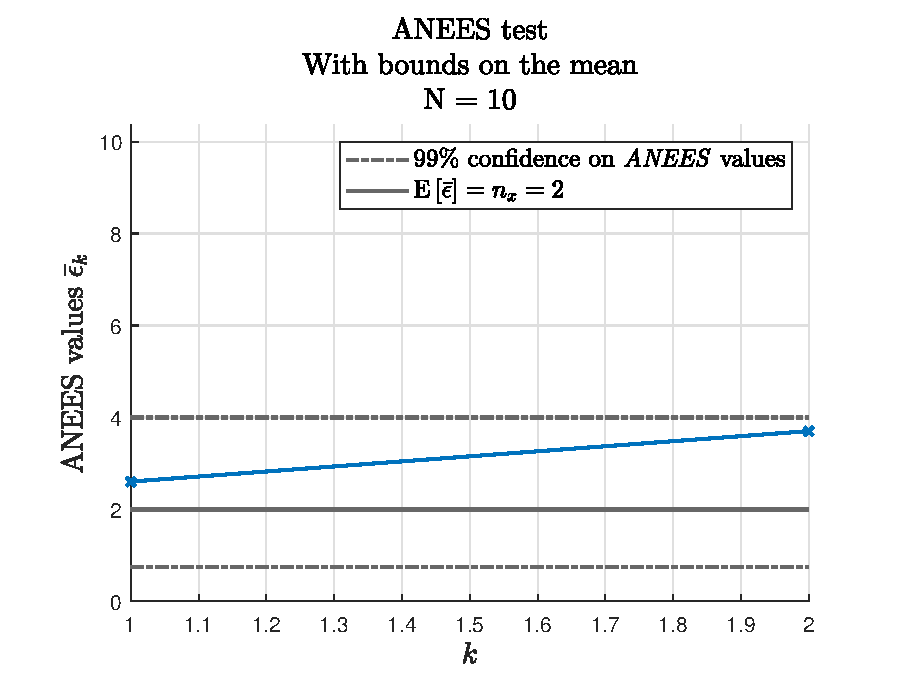
\includegraphics[width=\textwidth]{../figs/anees_N10.eps}
    \caption{$N=10$ trials.}
    \label{fig:anees_N10}
  \end{subfigure}
  %
  \begin{subfigure}{0.45\textwidth}
    \includegraphics[width=\textwidth]{../figs/anees_N100.eps}
    \caption{$N=100$ trials.}
    \label{fig:anees_N100}
  \end{subfigure}
  \caption{ANEES significance test on a Monte-Carlo trial using different number of trials $N$. The true covariance matrix $\mbfhat{P}_{1}^{\mathrm{t}}$ was used.}
  \label{fig:ANEES KF MCT true P}
\end{figure}

The conclusion of the results of the significance test presented in \figref{fig:ANEES KF MCT true P} is that the estimates (states and covariances) are \emph{not rejected}. This does \textbf{not} imply that the estimates must be accepted. To demonstrate this point, a false covariance matrix $\mbfhat{P}_{1}^{\mathrm{f}}$ will be used on state $\mbfhat{x}_{2}$ which has the value
\begin{align}
  \mbfhat{P}^{\mathrm{f}}_{1} 
        &= \bbm 1.99 & 0\\ 0 & 1/300 \ebm\inv\\
        \label{eq:false covariance 1}
        &= \bbm 0.5025 & 0\\ 0 & 300 \ebm.
\end{align}
It is clear that $\mbfhat{P}_{1}^{\mathrm{f}}$ is significantly different than the true value $\mbfhat{P}_{1}^{\mathrm{t}}$ in \eqref{eq:mbfhatP1 true value}; a good credibility test should detect that the covariance estimate is bad. 
\begin{blackBox}
  The values of $\mbfhat{P}^{\mathrm{f}}$ were specifically chosen to demonstrate a point that will be explained in Section~\ref{eq:When does the ANEES test fail}.
\end{blackBox}

The results from the ANEES significance test using the \emph{false} covariance matrix are presented in \figref{fig:anees_N100_falseCovariance}. At first glance, it seems that the estimates should be accepted since they fall within the uncertainty bounds. But that's a common fallacy since the ANEES significance test is a rejection-only test: failing to reject an estimate is should \emph{not} imply that the estimates are acceptable. Therefore, it could be dangerous conclude the consistency of estimates by solely relying on the ANEES test.

\begin{figure}[H]
  \centering
  \begin{subfigure}{0.45\textwidth}
    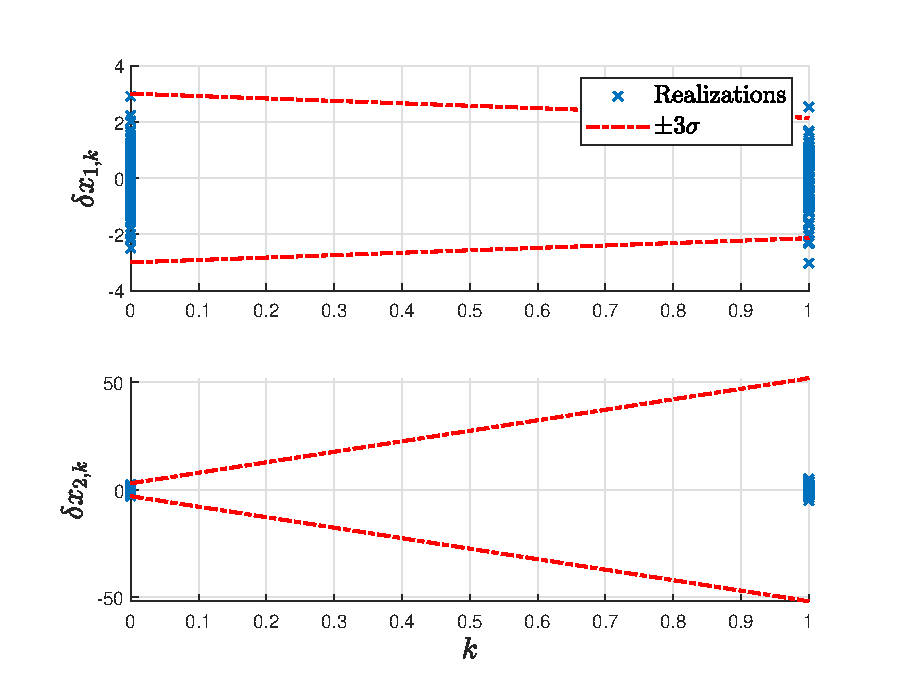
\includegraphics[width=\textwidth]{../figs/error_plots_N100_falseCovariance_scatter.eps}
    \caption{Error plots on the two states after Monte-Carlo trials.}
    \label{fig:error_plots_N100_falseCovariance_scatter}
  \end{subfigure}
  %
  \begin{subfigure}{0.45\textwidth}
    \includegraphics[width=0.8\textwidth]{../figs/anees_N100_falseCovariance.eps}    
    \caption{ANEES significance test.}
    \label{fig:anees_N100_falseCovariance}
  \end{subfigure}
  \caption{Error and ANEES plots on the KF estimates using the \emph{false} covariance matrix $\mbfhat{P}_{1}^{\mathrm{f}}$ \eqref{eq:false covariance 1}. This plot demonstrates an important point of the ANEES significance test: failing to reject an estimate does not imply the acceptance of the estimate.}
  \label{fig:false covariance plots 1}
\end{figure}

\subsection{When does the ANEES test fail?}
\label{eq:When does the ANEES test fail}
Let's look again at the NEES random variable given by
\begin{align}
  \rv{\epsilon}_{i} &\coloneqq \left( \mbfrv{x}_{i} - \mbfhatrv{x}_{i} \right)^{\trans}\mbshat{\Sigma}_{i}\inv\left( \mbfrv{x}_{i} - \mbfhatrv{x}_{i} \right).
\end{align}
Then the expected value of $\rv{\epsilon}_{i}$ is given by
\begin{align}
  \expect{\rv{\epsilon}_{i}} &= \expect{\left( \mbfrv{x}_{i} - \mbfhatrv{x}_{i} \right)^{\trans}\mbshat{\Sigma}_{i}\inv\left( \mbfrv{x}_{i} - \mbfhatrv{x}_{i} \right)}\\
                             &= \expect{\trace{\left( \mbfrv{x}_{i} - \mbfhatrv{x}_{i} \right)^{\trans}\mbshat{\Sigma}_{i}\inv\left( \mbfrv{x}_{i} - \mbfhatrv{x}_{i} \right)}}\\
                             &= \expect{\trace{\mbshat{\Sigma}_{i}\inv\left( \mbfrv{x}_{i} - \mbfhatrv{x}_{i} \right)\left( \mbfrv{x}_{i} - \mbfhatrv{x}_{i} \right)^{\trans}}}\\
                             &= \trace{\expect{\mbshat{\Sigma}_{i}\inv\left( \mbfrv{x}_{i} - \mbfhatrv{x}_{i} \right)\left( \mbfrv{x}_{i} - \mbfhatrv{x}_{i} \right)^{\trans}}}\\
                             &= \trace{\mbshat{\Sigma}_{i}\inv\expect{\left( \mbfrv{x}_{i} - \mbfhatrv{x}_{i} \right)\left( \mbfrv{x}_{i} - \mbfhatrv{x}_{i} \right)^{\trans}}}\\
                             &= \trace{\mbshat{\Sigma}_{i}\inv\mbs{\Sigma}_{i}},
\end{align}
which \textbf{under the null hypothesis} (if $\mbshat{\Sigma}_{i}=\mbs{\Sigma}_{i}$), then the expected value simplifies to
\begin{align}
  \expect{\rv{\epsilon}_{i}} &= \trace{\mbshat{\Sigma}_{i}\inv\mbs{\Sigma}_{i}}\\
                             &=\trace{\mbs{\Sigma}_{i}\inv\mbs{\Sigma}_{i}}\\
                             &= \trace{\eye}\\
                             &= n_{x}.
\end{align}
\begin{blackBox}
  Therefore, at the core of the ANEES test, at its core, is checking whether
  \begin{align}
    \label{eq:anees expression core}
    \trace{\mbshat{\Sigma}_{i}}\inv\mbs{\Sigma}_{i} &= n_{x}
  \end{align}
  is satisfied or not.
\end{blackBox}

Looking back at our example, the false covariance matrix $\mbfhat{P}_{1}^{\mathrm{f}}$ was chosen specifically so that the expression \eqref{eq:anees expression core} holds. That is,
\begin{align}
  \trace{{\mbfhat{P}_{1}^{\mathrm{f}}}\inv\mbf{P}_{1}^{\mathrm{t}}}
        &= \trace{
          \bbm 1.99 & 0\\ 0 & 1/300 \ebm
          \bbm 1 & -1\\-1 & 3 \ebm
        }\\
        &= \trace{
          \bbm 
          1.99 &  -1.99\\
          -0.0033  &  0.01
          \ebm
        }\\
        &= n_{x}.
\end{align}


\subsection{Another example}
By looking at \figref{fig:false covariance plots 1}, we might infer that looking at both the error plots \figref{fig:error_plots_N100_falseCovariance_scatter} as well as the ANEES plots \figref{fig:anees_N100_falseCovariance} would be sufficient to verify the consistency of the estimator. Unfortunately, spotting a ``bad'' estimator by looking at the error plots can be challenging. In this section, another example of a ``bad'' covariance matrix is presented. By looking at the error plots using this covariance matrix, it's not easy to spot that the estimated quantity is ``wrong''.

Here's another false covariance matrix
\begin{align}
  \mbfhat{P}_{1}^{\mathrm{f}} &= 
  \label{eq:false covariance 2}
  \bbm 
  2.0445   & 1.6162\\
  1.6162   & 4.7232
  \ebm\\
           &= \bbm 
  0.6705  & -0.2294\\
  -0.2294 &   0.2902
  \ebm\inv
\end{align}
such that
\begin{align}
  \trace{{\mbfhat{P}_{1}^{\mathrm{f}}}\inv\mbf{P}_{1}^{\mathrm{t}}}
        &= \trace{
          \bbm 
          0.6705  & -0.2294\\
          -0.2294 &   0.2902
          \ebm
          \bbm 1 & -1\\-1 & 3 \ebm
        }\\
        &= \trace{
          \bbm 
          0.8999  & -1.3588\\
          -0.5196 &   1.1001
          \ebm
        }\\
        &= 2\\
        &= n_{x}.
\end{align}

The error plots and the ANEES plot are presented in \figref{fig:false covariance plots 2}.

\begin{figure}[H]
  \centering
  \begin{subfigure}{0.45\textwidth}
    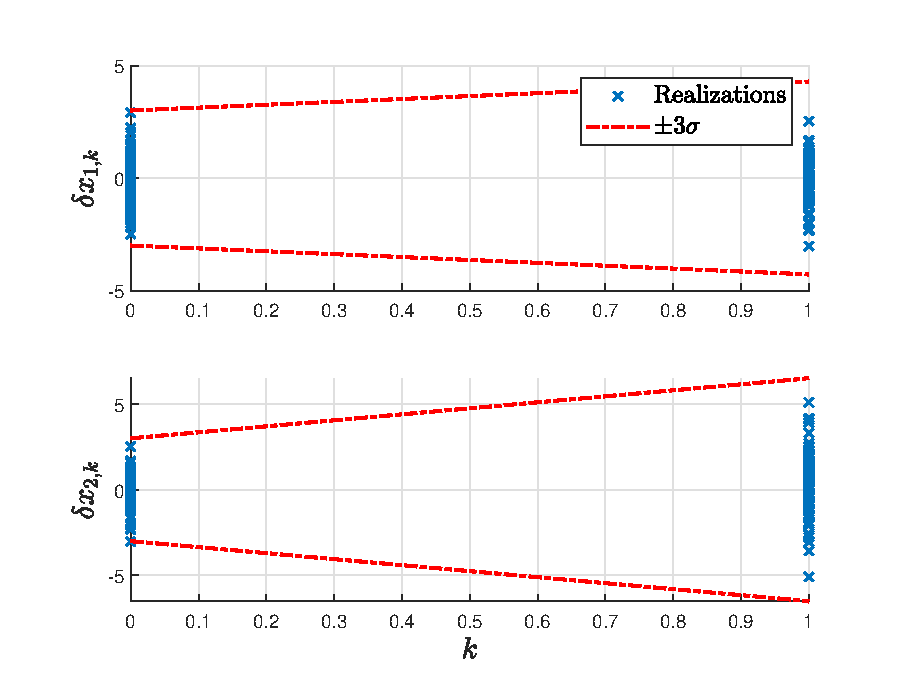
\includegraphics[width=\textwidth]{../figs/Phat_lmi/error_plots_N100_falseCovariance_scatter.eps}
    \caption{Error plots on the two states after Monte-Carlo trials.}
    \label{fig:error_plots_N100_falseCovariance_scatter 2}
  \end{subfigure}
  %
  \begin{subfigure}{0.45\textwidth}
    \includegraphics[width=0.8\textwidth]{../figs/Phat_lmi/anees_N100_falseCovariance.eps}    
    \caption{ANEES significance test.}
    \label{fig:anees_N100_falseCovariance 2}
  \end{subfigure}
  \caption{Error and ANEES plots on the KF estimates using the \emph{false} covariance matrix $\mbfhat{P}_{1}^{\mathrm{f}}$ \eqref{eq:false covariance 2}. This plot demonstrates an important point that looking at the error plots and the ANEES plots, alone, can be misleading and should not be used, alone, to verify the consistency of the estimates.}
  \label{fig:false covariance plots 2}
\end{figure}
%%%%%%%%%%%%%%%%%%%%%%%%%%%%%%%%%%%%%%%%%%%%%%%%%%%%%%%%%%%%%%%%%%%%%%%%%%%%%%%%%%%%%%%%%%%%%%%%%%%%
\printbibliography

\end{document}
